\section{Kinematics for the Da vinci robot}
This section is covering the derivation of one arm of the daVinci robot. 



\begin{figure}[H]
		\centering
		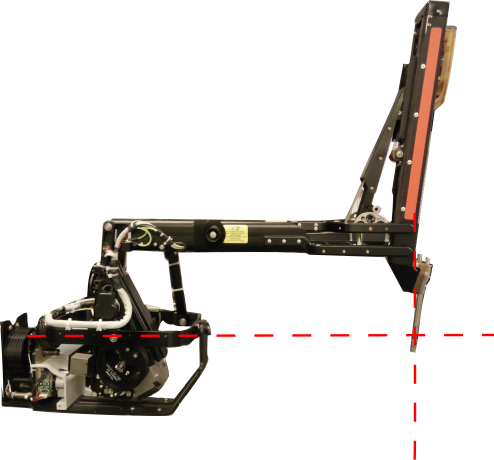
\includegraphics[width=1\linewidth]{Hand_davinci_robot.png}
		\caption{The da Vinci hand with dotted line, where the cross section is the stationary reference for the hand.}
		\label{fig:da_ha_en}
\end{figure}





\begin{table}[H]
\centering
\begin{tabular}{|l|l|l|l|l|}
\hline
 $j_i$ 	  & $a_i$    & $d_i$ & $\alpha_i$ 		 & $\theta_i$ 			   	 \\ \hline
 1  	  &  $0$     & $0$ 	 & $-\frac{\pi}{2}$	 		 & $q_1$ 			    	 \\ \hline
 2  	  &  $0$   	 & $0$ 	 & $ \frac{\pi}{2}$ 	 & $\frac{\pi}{2}+q_2$ 		 \\ \hline
 3  	  &  $0$	 & $d_3$ & $0$ 		 		 & $0$ 					 \\ \hline
\end{tabular}
\caption{The DH notations for the\newline Geomagic Touch}
\label{tab:kin_geo}
\end{table}



\begin{sidewaysfigure}
		\centering
		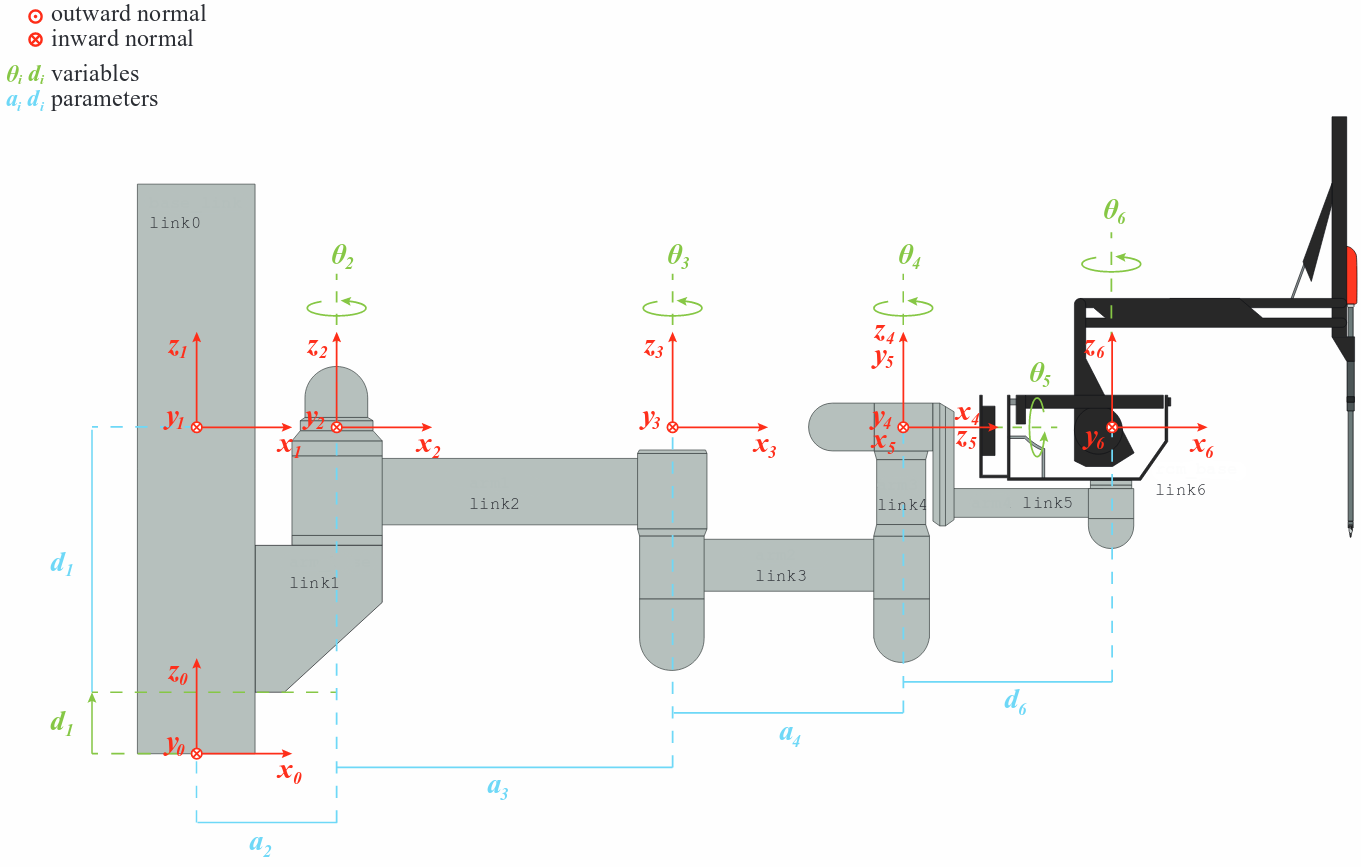
\includegraphics[width=0.9\linewidth]{da_arm.png}
		\caption{Show different joints and their attached frame coordinate}
		\label{fig:da_ha_en}
\end{sidewaysfigure}


%stolen from page 108:
%projekter.aau.dk/projekter/files/213514652/Safety_in_Automated_Surgery_with_the_da_Vinci_Robot.pdf

\todo{Better resulution}
\todoc{Do we have to draw this our self or is it okay just to make a ref to stolen location}
\begin{sidewaysfigure}
		\centering
		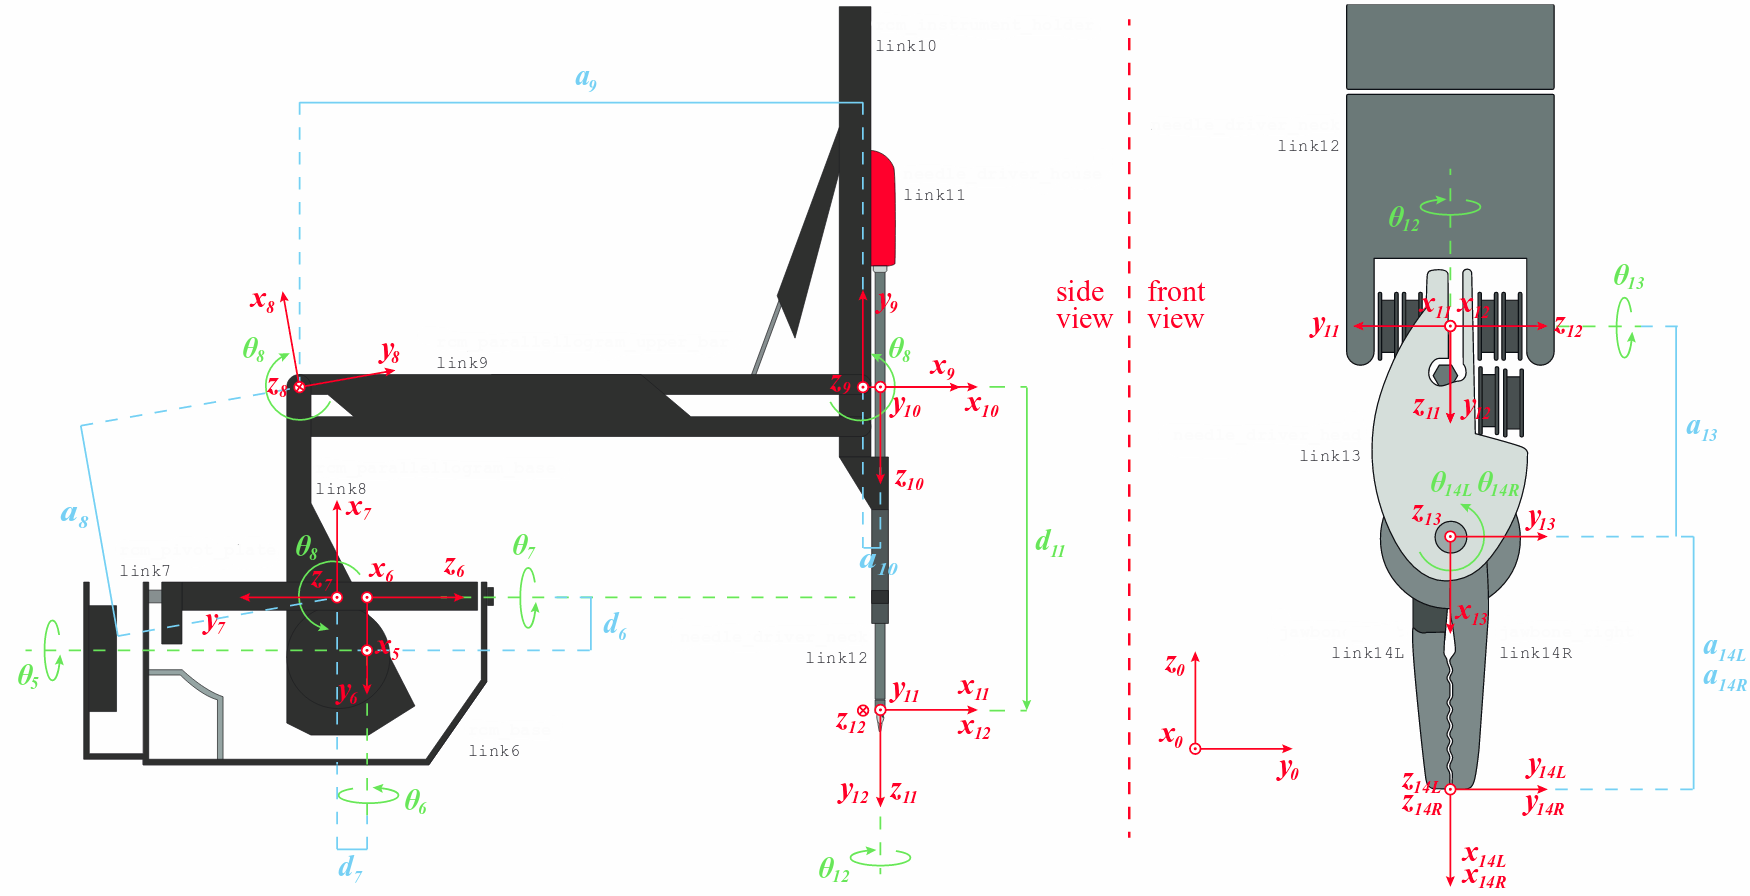
\includegraphics[width=1\linewidth]{Davinci_hand_endo.png}
		\caption{Show different joints and their attached frame coordinate}
		\label{fig:da_ha_en}
\end{sidewaysfigure}

